\emph{Valoració}

La practica ha resultat molt interessant, pero al principi va costar un poc
adequar l'entorn de treball. Per tal de poder emprar la llibreria i el simulador
\emph{MobileSim} en la \emph{Debian} que empram normalment
va requerir compilar-ho de nou, cosa que generà algun problema de dependències
però va quedar sobradament compensat per la comoditat de no haver d'emprar una
màquina virtual.

Cal destacar que el \emph{Mapper3Basic} i el \emph{MobileSim} són de gran ajuda 
a l'alumne i permeten fer simulacions per res comparables amb la primera
pràctica del braç robot que resulten vitals per el desenvolupament de la
pràctica.

La llibreria \emph{Aria} en general esta força bé i és bastant intuïtiva, rara 
vegada s'ha hagut de cercar informació addicional que no figurés a la API.

Per altra banda s'ha de mencionar que el \emph{C++} ens ha suposat algun mal de 
cap, sobretot en l'àmbit de visibilitat dels procediments i l'ús de punters. En
aquest sentit ens hagués agradat tenir temps per provar de fer la pràctica amb
\emph{Python} ja que l'\emph{Aria} en te uns \emph{bindings}. L'únic fet que ens
tirà endarrere es que no sabíem si funcionaria el simulador i que possiblement
la llibreria no està insta\lgem al robot real.

També ens han portat molts mal de cap el trobar valors adequats per cada una de 
les ponderacions i llindars. Sovint ens trobàvem que amb certa combinació de
llindars, especialment als de \emph{heading} el robot podia quedar fent voltes
sobre si mateix si el punt on havia d'anar era proper al punt actual però havia
de fer un canvi d'orientació. 

\begin{figure}[H]
\begin{center}\label{headingthproblem}
 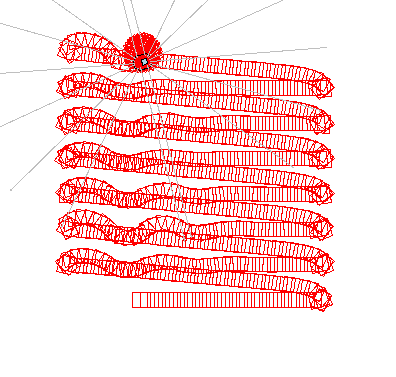
\includegraphics[width=0.5\textwidth]{diagrames/figures/voltes.png}
 % ordreRotacions.png: 1286x768 pixel, 150dpi, 21.77x13.00 cm, bb=0 0 617 369
\end{center}
  \caption{Problema amb llindar de heading}
\end{figure}

Atribuirem aquest problema a que el robot inicia el moviment abans d'estar 
orientat però donat que la proximitat es molt gran no acaba d'orientar-se mai.

Tot i així i encara que ens hagués agradat implementar alguna cosa més
consideram la pràctica acabada i assolits els coneixements bàsics i que per tant
les implementacions que tenim en ment i figuren en l'apartat d'ampliacions es
converteien en rutina ja que no requereixen conceptes nous sinó simples
combinacions i modificacions sobre l'arquitectura i rutines ja implementades.